\chapter{Метод случайных деревьев}\label{chapter:2}

Метод случайных деревьев, предложенный в \cite{Broadie1997}, ищет решение проблемы оптимального времени остановки и оценивает истинное значение цены Американского опциона (в отличие от метода параметрических приближений).

Известно, что точное значение цены А.о. может быть найдено с помощью методов динамического программирования, и оценки из \cite{Broadie1997} используют эти методы. Задача динамического программирования --- это задача \eqref{eq:common_recursive_statement}. В ней для численной реализации математическое ожидание заменяется на среднее арифметическое всех или части оценок на следующем шаге алгоритма (и именно эта замена является источником смещения получаемых оценок). Таким образом, мы видим, что рекуррентное выражение содержит оператор, который связывает значение в $k$ момент времени с $b$ значениями в последующий момент времени. Именно это приводит нас к визуализации задачи в виде дерева состояний, представленного на рис. \ref{fig:exponential_tree}.

С другой стороны, известно, что подобный же приём используется при решении нелинейных уравнений, в которых присутствует полиномиальная нелинейность

\par Вместо того, чтобы строить оценку, каким-либо образом стремящуюся к $V_0\left(X_0\right)$, мы построим две функции, являющиеся смещёнными вверх и вниз состоятельными оценками $V$, (в \cite{Broadie1997} приведено доказательство отсутствия несмещённой оценки для $V_0\left(X_0\right)$). Пусть $\Vhat\left(b\right)$ и $\vhat\left(b\right)$ --- такие оценки, зависящие от некоторого параметра $b$, сходящиеся к $V$ при $b\to\infty$.
\par Метод случайного дерева основан на моделировании случайной цепи $X_0, X_1, \ldots X_m$. Зафиксируем параметр ветвления $b$. Из исходного состояния $X_0$ смоделируем $b$ независимых следующих состояний $X_1^1, X_1^2, \ldots X_1^b$, все с условием $X_1$. Для каждого $X_1^i$ снова смоделируем $b$ независимых последующих состояний $X_2^{i1}, \ldots X_2^{ib}$. На $m$-ом шаге будем иметь $b^m$ состояний, и это и есть источник основного недостатка этого метода --- его экспоненциальной алгоритмической сложности. Пример получающегося дерева состояний приведён на \ref{fig:exponential_tree}.
\begin{figure}
	\centering
	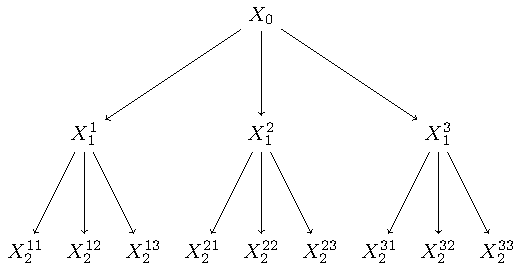
\includegraphics[width=0.7\textwidth]{exponential_tree}
	\caption{Дерево состояний для $b = 3, m = 2$}
	\label{fig:exponential_tree}
\end{figure}
\section{Оценка сверху}
	% \par Определим $\Vhat_i^{j_1, j_2 \ldots j_i}$, вдохновляясь \ref{eq:option-recursive}. В последних вершинах (листьях) дерева зададим
	\par Используя \eqref{eq:common_recursive_statement}, зададим оценку в терминальных вершинах дерева равной известному значению функции выплат
	\begin{equation}\label{eq:upper-terminal}
		\Vhat_m^{j_1 \ldots j_m} = h_m\left(X_m^{j_1 \ldots j_m}\right),
	\end{equation}
	в нетерминальных вершинах будем пользоваться результатами вычислений на предыдущем шаге
	\begin{equation}\label{eq:upper-node}
		\Vhat_i^{j_1 \ldots j_i} = \max \left\lbrace h_i \left( X_i^{j_1 \ldots j_i} \right), \frac{1}{b} \sum_{j = 1}^b \Vhat_{i+1}^{j_1 \ldots j_i j}\right\rbrace .
	\end{equation}
	\par Другими словами, оценка сверху --- это просто результат обхода дерева в глубину с присвоением каждой ветви дерева одинакового веса.
	\par Смещённость оценки вверх и её состоятельность доказывается с помощью индукции:
	\begin{theorem}
		$\forall i \in 1:n$
		\begin{equation*}
		\mathsf{E}\left[\Vhat_i^{j_1\ldots j_i}|X_i^{j_1\ldots j_i}\right] \geq V_i\left(X_i^{j_1\ldots j_i}\right)
		\end{equation*}
	\end{theorem}
	\begin{proof}
		\par В листьях дерева неравенство выполняется как равенство по определению.
		\par Докажем, что если утверждение теоремы выполняется на $i+1$ шаге, то оно выполняется и на $i$. По определению
		\begin{equation*}
		\ev\left[\Vhat_i^{j_1\ldots j_i}|X_i^{j_1\ldots j_i}\right] = \ev\left[ \max\left\lbrace h_i\left(X_i^{j_1\cdots j_i}\right), \frac{1}{b}\sum_{j = 1}^b \Vhat_{i+1}^{j_1 \ldots j_i j}\right\rbrace | X_i^{j_1\cdots j_i} \right],
		\end{equation*}
		с помощью неравенства Йенсена ($\varphi\left(\ev\left[X\right]\right) \leqslant \ev\left[\varphi(X)\right]$) это можно оценить как
		\begin{equation*}
		\ev\left[ \max\left\lbrace h_i\left(X_i^{j_1\cdots j_i}\right), \frac{1}{b}\sum_{j = 1}^b \Vhat_{i+1}^{j_1 \ldots j_i j}\right\rbrace | X_i^{j_1\cdots j_i} \right] \geq \max\left\lbrace h_i\left(X_i^{j_1\cdots j_i}\right), \ev\left[ \frac{1}{b}\sum_{j = 1}^b \Vhat_{i+1}^{j_1 \cdots j_i j} | X_i^{j_1\cdots j_i} \right] \right\rbrace,
		\end{equation*}
		в силу того, что $\forall \, j \in 1:b \quad X_{i+1}^{j_1\cdots j_i j}$ - независимые одинаково распределённые случайные величины (и их математическое ожидание одинаково), $\ev\left[ \frac{1}{b}\sum_{j = 1}^b \Vhat_{i+1}^{j_1 \cdots j_i j} \right] = \frac{1}{b}\sum_{j = 1}^b \ev\Vhat_{i+1}^{j_1 \cdots j_i j} = \ev\Vhat_{i+1}^{j_1 \cdots j_i 1}$, а в силу индукционного предположения
		\begin{equation*}
		\begin{aligned}
		\max\left\lbrace 
			h_i\left(X_i^{j_1\cdots j_i}\right), 
			\ev\left[ \Vhat_{i+1}^{j_1 \cdots j_i 1} | X_i^{j_1\cdots j_i} \right] 
		\right\rbrace &\geq \max \left\lbrace 
			h_i\left(X_i^{j_1\cdots j_i}\right),
			\ev\left[V_{i+1}\left(X_i^{j_1\ldots j_i 1}\right)\middle\vert X_i^{j_1\ldots j_i}\right]
		\right\rbrace \\ &\geq V_i\left(X_i^{j_1\ldots j_i}\right).
		\end{aligned}
		\end{equation*}
		Таким образом, $\ev\left[\Vhat_i^{j_1\ldots j_i}|X_i^{j_1\ldots j_i}\right] \geq \max \left\lbrace h_i\left(X_i^{j_1\cdots j_i}\right), V_i\left(X_i^{j_1\ldots j_i}\right) \right\rbrace$
	\end{proof}
	\begin{theorem}\label{thm:consistency} Оценка $\Vhat$ асимптотически состоятельна, то есть
		$$\Vhat_i^{j_1\ldots j_i} \underset{b\to\infty}{\overset{\mathsf{P}}{\to}} V_i\left(X_i^{j_1\ldots j_i}\right)$$
	\end{theorem}
	\begin{proof}
		\par В листьях дерева это очевидно ($\Vhat_m^{j_1 \ldots j_m} = h_m\left(X_m^{j1 \ldots j_m}\right) = V_m\left(X_m^{j1 \ldots j_m}\right)$ по определению). Предположим, что $\Vhat_{i+1}^{j_1\ldots j_i} \underset{b\to\infty}{\overset{\mathsf{P}}{\to}} V_{i+1}\left(X_i^{j_1\ldots j_i}\right)$. 

		Обозначив $\Vhat_k = \Vhat_k^{j_1\cdots j_k}$, $\Vhat_{k+1}^i = \Vhat_k^{j_1\cdots j_k i}$ для некоторой случайной последовательности $j_1\cdots j_k$, $\norm{\xi}_{X_k} = \left(\ev\left(\xi^p\middle\vert X_k\right)\right)^{1\over p}$, получим на $k$-м шаге
		\begin{multline*}
			\norm{\Vhat_k(b) - V\left(X_k\right)}_{X_k} = \\ 
			= \norm{
				\maxset{
					h_k\left(X_k\right), \frac{1}{b}\sum_{i=1}^b \Vhat_{k+1}^i(b)
				} - \maxset{
					h_k\left(X_k\right), \ev\left(V\left(X_{k+1}\right) \middle\vert X_k\right)}
			}_{X_k} \leq \\
			\leq \norm{\frac{1}{b}\sum_{i=1}^b \Vhat_{k+1}^i(b) - \ev\left(V\left(X_{k+1}\right) \middle\vert X_k\right)}_{X_k} \leq \\
			\leq \norm{
				\frac{1}{b}\sum_{i=1}^b  
				\left(\Vhat_{k+1}^i(b) - V_{k+1}\left(X_{k+1}^i\right)\right)
			}_{X_k} + \\ +\norm{
				\frac{1}{b}\sum_{i=1}^b   V_{k+1}\left(X_{k+1}^i\right) - 
				\ev\left(V\left(X_{k+1}\right) \middle\vert X_k\right)
			}_{X_k}.
		\end{multline*}

		Второе слагаемое является разностью суммы реализаций независимых (при данном $X_k$) случайных величин и математического ожидаемого слагаемых этой суммы и сходится по закону больших чисел. Для первого же применяется индукционное предположение, в итоге $$\norm{\Vhat_k(b) - V\left(X_k\right)}_{X_k} \underset{b\to\infty}{\to} 0.$$
	Сходимость по норме даёт нам сходимость по вероятности, тем самым доказывая, что оценка $\Vhat$ состоятельна. Более подробное доказательство можно найти в \cite{Broadie1997}.
	\end{proof}
\section{Оценка снизу}
	\par Значения оценки сверху в каждый момент времени --- это выбор максимума из стоимости опциона при его немедленном исполнении и математического ожидания стоимости удержания опциона. Но стоимость удержания опциона рассчитывается, исходя из дочерних узлов дерева состояний актива,то есть оценка сверху рассчитывается, опираясь на информацию о будущем. Чтобы убрать ошибку, связанную с этим, необходимо отделить механизм принятия решения о исполнении или удержании опциона от значений, полученных после принятия решения об удержании опциона.
	\par В более общей (и более короткой) постановке --- необходимо оценить $\max\left\lbrace a, \ev Y \right\rbrace$ с помощью $b$ независимых одинаково распределённых реализаций случайной величины $Y$ для некоторой константы $a$ и случайной величины $Y$. Оценка $\max\left\lbrace a, \bar{Y}\right\rbrace$ (где $\bar{Y}$ --- среднее значение выборки) является оценкой сверху, так как $\ev\max\left\lbrace a, \bar{Y}\right\rbrace \geq \max\left\lbrace a, \ev\bar{Y}\right\rbrace = \max\left\lbrace a, \ev Y\right\rbrace$, что и было использовано в построении оценки сверху.
	\par Разделим множество реализаций $\left\lbrace Y_i \right\rbrace _{i=1}^b$ случайной величины $Y$ на два независимых подмножества и вычислим их средние значения $\bar{Y}_1$ и $\bar{Y}_2$. Если положить
	\begin{equation}
	\vhat = \begin{dcases*}
		a, & если $\bar{Y}_1 \leqslant a$, \\
		\bar{Y}_2, & иначе,
	\end{dcases*}
		% \begin{array}{l l}
		% 	a, & \, \text{если } \bar{Y}_1 \leqslant a, \\
		% 	\bar{Y}_2, & \, \text{иначе,} 
		% \end{array}\right.
	\end{equation}
	мы отделим процесс принятия решения о исполнении или удержании опциона от оценки стоимости (за решение будет отвечать $\bar{Y}_1$, за оценку - $\bar{Y}_2$). При этом оценка $\vhat$ является оценкой снизу:
			\[
				\ev\vhat = \mathsf{P}\left(\bar{Y}_1 \leqslant a\right)a + \left( 1 - \mathsf{P}\left(\bar{Y}_1 \leqslant a\right) \right)\ev Y \leqslant \max\left\lbrace a, \ev Y \right\rbrace
			\]
			
	В оригинальной работе \cite{Broadie1997} была исполоьзована немного другая оценка. Пусть <<отвечающим за принятие решения>> подмножеством будут все реализации, кроме одной, а <<оценивающее>> множество будет состоять из одной оставшейся реализации. Возьмём математическое ожидание этой величины, т.е. положим в листьях дерева значение оценки
    \begin{equation}\label{eq:lower-terminal}
		\vhat_m^{j_1 j_2 \cdots j_m} = h\left( X_m^{j_1 j_2 \cdots j_m}\right),
	\end{equation}
	а для промежуточных узлов определим
    \begin{equation}
        \vhat_{ik}^{j_1 j_2 \cdots j_i} = \left\lbrace
		    \begin{array}{l l}
			    h\left( X_i^{j_1 j_2 \cdots j_i}\right), & \, \text{если } \frac{1}{b-1}\sum_{j=1, j\not= k}^b \vhat_{i+1}^{j_1 j_2 \cdots j_i j} \leq h\left(X_i^{j_1 j_2 \cdots j_i}\right) \\
			    \vhat_{i+1}^{j_1 j_2 \cdots j_i k}, & \, \text{иначе} 
		    \end{array}\right.
    \end{equation}
    и оценку положим равной 
    \begin{equation}\label{eq:lower-node}
    	\vhat_i^{j_1 j_2 \cdots j_i} = \frac{1}{b}\sum_{k=1}^b \vhat_{ik}^{j_1 j_2 \cdots j_i}.
    \end{equation}

	Доказательства смещённости и состоятельности нижней оценки аналогичны вышеприведённым для оценки сверху и также могут быть найдены в \cite{Broadie1997}.

	Таким образом, мы имеем дерево с $\sum_{k=1}^m b^k = \frac{b\left(b^m-1\right)}{b-1} = O\left(b^m\right)$ вершинами. Несмотря на то, что потребление памяти в процессе работы алгоритма можно держать в рамках $O\left(bm\right)$ (структура алгоритма подразумевает обход дерева в глубину с сохранением только присущих обходимой траектории значений), анализа требуют все $O\left(b^m\right)$ вершин, что означает экспоненциальный рост временной сложности алгоритма. Следовательно, об устремлении $m\to\infty$ в изначальной форме алгоритма речь идти не может.
